\documentclass{article}

% See http://mirror.its.dal.ca/ctan/macros/latex/contrib/appendix/appendix.pdf for more appendix info
\usepackage[page,toc,title,titletoc]{appendix}
\usepackage[
	backend=bibtex,
	natbib=true,
	style=numeric,
	sorting=none
]{biblatex}

% Margins - see http://mirror.its.dal.ca/ctan/macros/latex/contrib/geometry/geometry.pdf for more info
\usepackage[left=3cm,top=3cm,right=3cm,bottom=3cm]{geometry}
\usepackage{graphicx}
\usepackage{lipsum}
\usepackage{pgfgantt}

% Temporary bugfix for BibTeX
% Found at http://tex.stackexchange.com/a/311428
\makeatletter
\def\blx@maxline{77}
\makeatother

\bibliography{proposal}

\title{SYSC4907 Project Proposal: \\ Sensor-Based Access Control System}
\author{
	Craig Shorrocks \\
	100887781
	\and
	Jessica Morris \\
	100882290
	\and
	Richard Perryman \\
	100887250
}

% Might be better to use the last date we edit this on,
% but for now I was too lazy to keep updating this
\date{\today}

\begin{document}

\maketitle

\begin{center}
Supervisors: Shikharesh Majumdar and Chung-Horng Lung
\end{center}

\pagebreak

\tableofcontents

\pagebreak

\section{Objective}

As technology becomes more and more prevalent in our lives, our identities become increasingly intertwined with the
technologies that we use daily. This melding has become extremely prevalent in some areas. Some example areas are
professional networking with LinkedIn, and banking, with the advent of online account management. Over half of all
smartphone users have used mobile banking~\autocite{MOBILEBANKING}. This popularity may be derived
from how convenient and secure the online handling money of is. However, certain aspects of our day to day lives
haven't yet been graced by the benefits of electronic security and automation.

Physical locks and keys are still widely used for several tasks where electronic locks could be used instead. House
locks, bicycle locks, and locker locks are frequently physical locks. Changing to electronic locks could help streamline
all of these locks, reducing the number of keys to remember and improving security by reducing the likelihood that the
key could be faked by an attacker. This would also reduce the risk of misplacing keys, as a digital key can be backed 
up for use on another device. Some applications for this have already been found: for example, Walmart has a system 
where customers can order products to be placed in lockers with electronic keys called Grab-and-Go~\autocite{WALMART}. 
Such a system greatly reduces the work involved in getting a key to the customer, as a PIN can be sent and received 
electronically. It also increases the security of the lockers by reducing the number of points of failure.

This proposal outlines a system, a Sensor-Based Access Control System~(SBACS), that will expand upon such a concept to 
further tie security and identity to the electronics we use most: our phones. Using technologies like near-field 
communication~(NFC) sensors and quick response~(QR) codes, the identity associated with a phone can be used as 
identification for anything requiring access control. This represents a huge advantage with respect to convenience, and 
it would even further lower the number of possible failure points in security. In addition, with modern mobile devices 
being automatically backed up over-the-air, recovering an identity when a device is lost or stolen can be accomplished 
easily and securely.

\section{Background}

NFC is a form of short-range, low-power communication used by devices such as smartphones and tablets. NFC is a fast
and convenient method to exchange small amounts of data, as it does not require any steps to set up a connection. The 
active device uses magnetic induction to create a current in the information-holding passive device. The
passive device responds by modulating the EM field coming from the active device. The active device then reads and
converts the modulations into useful data~\autocite{NFCORG}. This scenario is a NFC communication in passive mode. Two
smartphones may both act as passive and active devices, allowing them to exchange data through a call-and-response procedure,
also known as communication in active mode.

NFC is being increasingly used to smarten up passive information delivery systems such as business cards, and posters.
Brief data such as contact information, URLs, or credentials may be written to a passive NFC device, such as a smart
tag~\autocite{NFCFORUMWHATIS}, and read by any NFC-enabled mobile device. These mobile devices can also be used to
replace credit cards in contactless exchanges. In fact, NFC payments may be more secure than payment with a card, as
each point in the transaction requires the device and the reader to exchange an encrypted password, and the transaction
 must be approved by the device's user before the device sends payment information~\autocite{NFCPAYMENT}.

Because of the close range required for an exchange, NFC has inherent protections against attackers. An NFC exchange
can only be reliably eavesdropped from a distance of approximately 10 metres or less if the interaction is between two 
active devices, dropping to 1 metre if the interaction is a passive communication ~\autocite{NFCSECURITY}. This, along 
with some other facts, makes a man-in-the-middle attack nearly impossible to accomplish in a real-world 
scenario~\autocite{NFCSECURITY}. These attacks may be protected against by establishing a secure channel, by using 
symmetric-key encryption or other secret-sharing method. For these reasons, NFC is a reliable method to pair a smart 
device with an electronic lock system.

\section{Methods}

To realise this Access Control System, several separate components will need to communicate with each other. An
application for the mobile devices will enable the device to communicate with the rest of the system. An application
programming interface~(API) running on a server will expose the the interactions between customers, administrators and
the physical components. This API will be structured as a framework, allowing for easy access by developers seeking to
make similar applications. A unit of authentication in the system will be represented by an expiring token that contains
validation along with the associated user. A database will store relevant information to be accessed by the other
components. Together, along with the physical components of the locks, these subsystems will power the Sensor Based
Access Control System.

At the hardware level, the system will consist of several components. A Raspberry Pi will provide the main point of 
communication between the software applications (user app, administration) and the hardware, such as sensor modules for 
access. It will verify tokens provided by the sensor modules against the values stored in the database, and send "open" 
or "close" signals to an electronic strike lock when necessary. An Arduino microcontroller, connected to the Pi via 
USB, will act as an operator for the sensor modules, performing message-passing between the modules and the Pi. Various 
types of sensor modules, powered by any small microcontroller, send identity tokens to the Arduino. The primary access 
module provided with the system will be a NFC module, whose prototype will be powered by a Adafruit Feather board with 
a Adafruit PN532 NFC shield.

\subsection{Online Order Secure Pickup}

With online shopping becoming more popular~\autocite{CUSTORA}, the hassle of being physically present to shop in stores 
can be eliminated by allowing customers to make an order and payment online, then pick up their products at the store 
using a SBACS-secured storage container. After a customer's order has been confirmed by the store to be packed 
and ready for pick-up, the store's system administrator sends one or several one-time-use authentication tokens 
to the customer's SBACS app on their smartphone. When the customer arrives at the store to pick up their items, 
they can gain access to the storage container assigned to them by using the authentication token(s) they had previously 
received, such as a hand-shaking code to use with the NFC module of the system. When the tokens have been used and the 
customer has retrieved their order, the storage container is assigned new tokens so that it may be used for another 
order, without wrongfully granting re-access to the previous customer.

A strong advantage of this system over existing ones, such as Walmart's Grab \& Go, is that it creates a digital 
fingerprint using a combination of authentication methods supported by the SBACS, which is more difficult to 
break via brute force than a 6-digit PIN~\autocite{WALMART}. In addition, with the entire process of shopping being 
expedited, customers will spend less time in stores and parking lots, leading to less congestion due to vehicle 
traffic. This system will also grant customers with mobility or vision impairments increased personal autonomy, as 
they will be able to retrieve their goods with less aid from store employees than traditional shopping allows. Customers
with impairments can perform their shopping online using their accessibility software, such as text-to-speech, instead 
of calling the store to request that an employee retrieve their goods. When the customer receives confirmation of their 
order and authentication tokens, they can access their assigned SBACS-secured locker in the store themselves, using 
their usual aids instead of occupying a store employee.
\hfill \break

\noindent A visualisation of some of the functionality of the system is available in Appendix A - UML.

\subsection{Central Mail Package Pickup}

Some parcels are too large to fit in a regular mail box, and must be delivered in person. Many delivery services only 
operate during standard work hours, while many people that need to accept the delivery will not be home. In these cases 
where packages cannot be stored in a mail box, and cannot be accepted by the recipient, these packages often go to an office 
of the delivery service. The recipient must then go to pick up their package at the office. This is counter-productive, 
as the customer has paid for the delivery, and now they are forced to go out of their way to get their item, which has not 
been delivered to their desired location.

% Mention already existing central holding places (community mailboxes)
In some places, Canada Post already has community mailboxes, which have a box for larger parcels. The problem with this
is that it is only usable for parcels that are being delivered with Canada Post, but there are other parcel delivery
services as well that are unable to make use of this. This community mailbox also uses a physical key to open this box,
where they leave the key in the customer's normal mailbox, then they use that key to open the parcel box, then they must 
return the key by dropping it in a mail delivery slot. This involves the need for the physical keys, and requires staff to
physically find the keys for the parcel box among the other mail that is in the delivery slot. The Sensor-Based Access 
Control System would eliminate the need for these physical keys, and would allow more delivery services to make use of
the same boxes, ensuring that it is most convenient for the customers.

This system could be used to access parcel boxes, which would allow the delivery to be placed in a box that would fit 
the parcel. These boxes could be set up in an area where they are close to many customers, allowing them to quickly 
pick up their parcel without going all the way to the local office. The delivery person would grant access to the 
customer, then place the parcel in the box. Then the customer could be notified through the application that there is a 
parcel ready to be picked up. When the customer arrives at the box, they can use the application to open the parcel 
box, and receive their package.

% C - Added a bit about expiry, is that enough?
Throughout this process, the system could make use of the registrations that have been set up for the central mail
box. The user set up as the deliverer would be able to send updates to the system on the status of the package, allowing
the recipient user to better know when their package would arrive. Further, the system could be configured such that the
system would notify the user when the package had not been picked up after a certain time had elapsed since it was
dropped off. This information could also be exposed to the people who manage the central mail box, allowing them to
determine the status of their boxes, informing them of potential problems, such as a package that has been languishing
for too long in the same box. If the package is not picked up after a given amount of time, the system would notify the
customer that the package will no longer be available to be picked up, and alternate options will be given. This would
also lead to an expiry of the customer's registration to the box, so they will no longer be able to open the box.

\subsection{Long Term Storage}

The Sensor-Based Access Control System also has applications for long term storage companies, such as Dymon. For these 
companies, the system could be viewed as an overall manager of customer storage. The system's registrations can be used 
to provide additional services for specific storage spaces. The system will also expose much of the administrative 
tasks that the company will need to provide.

The system, using its multiple step authentication, would allow the company to advertise greater security. Along with
similar methods to those described in the above use cases, the system could be configured to require biometrics, such
as fingerprints or facial recognition, as a form of authentication. By combining these metrics, the system would greatly
reduce the potential for attack by strengthening the potential failure points of the identification process.

Once a customer has a storage space reserved and has set up their identification, the registration could be configured
to expose additional features. An example feature would be a live video stream of the contents of the storage space.
This would allow the customer to verify that the contents of the space had been correctly stored, for example after
requesting that the company switch their locker.

Another additional feature would be the option to log items that are stored in the storage space. Through the system, the
customer would be able to note which items they are adding or removing from the storage space, which would later allow the
customer to remotely access a list of the items in the storage space, so they do not have to remember all of the contents.
This provides a different view of the stored contents on top of the video stream mentioned above. This list could also be
searchable or contain images of the items, to make the list easier to use.

The system would also provide the ability to dynamically give certain users access to the storage room. This would allow
a storage room to be communally owned by the members of a conglomerate, for example a company. This would ease the
process by which multiple people may access the storage space while also ensuring that control of the storage was held
centrally. More privileged users would be able to allow temporary access to less privileged users for a given time
period. All of the attemped authentications would also be logged and made available to certain users, creating a
reliable paper trail.

\subsection{Service Provider}

Since one of the main goals of the Sensor-Based Access Control System is to allow for a user to share their identities
between different locks, a logical application of the system is a service provider. A service provider could sell the
installation and management of the system to other companies that might want to make use of it, such as Walmart or
Dymon mentioned above.

This would benefit the end users as they would be able to share their identities amongst the service providers' various
customers. This would allow someone to sign up for a locker at Walmart, and later reuse all the work that they did to
set that up to unlock their central mail box or their home. This shared identity would allow people to remember fewer
passwords and generally have fewer physical keys.

Customers purchasing the services for the SBACS would save any technical work associated with installing the system.
The service provider would be able to manage the databases, servers and any customer complaints or feedback. Providers
would also take care of sharing end user identities which would even further increase how much time end users could save
This incentivises companies to make use of a service provider, as it makes the resulting system more attractive to
potential customers as well as reducing the overall cost of setting up the system.

\newpage % Just to make the formatting nicer
\section{Time Table}

% Gantt chart documentation available at http://ctan.mirror.rafal.ca/graphics/pgf/contrib/pgfgantt/pgfgantt.pdf
\begin{figure}[!ht]
\centering
\begin{ganttchart}[
	x unit=0.85cm,
	y unit chart=0.75cm,
	hgrid, vgrid,
	bar label font=\footnotesize,
	group label font=\footnotesize,
	title label font=\footnotesize
]{1}{15}
	\gantttitle{Fall Term}{15} \\
	\gantttitle{09/11}{1}
	\gantttitle{09/18}{1}
	\gantttitle{09/25}{1}
	\gantttitle{10/02}{1}
	\gantttitle{10/09}{1}
	\gantttitle{10/16}{1}
	\gantttitle{10/23}{1}
	\gantttitle{10/30}{1}
	\gantttitle{11/06}{1}
	\gantttitle{11/13}{1}
	\gantttitle{11/20}{1}
	\gantttitle{11/27}{1}
	\gantttitle{12/04}{1}
	\gantttitle{12/11}{1}
	\gantttitle{12/18}{1} \\
	\ganttbar{Draft proposal}{1}{2} \\
	\ganttbar{Final proposal}{2}{4} \\
	\ganttbar{Preliminary design}{3}{6} \\
	\ganttbar{Hardware prototype}{5}{10} \\
	\ganttbar{Software prototype}{5}{10} \\
	\ganttbar{Preliminary testing}{8}{12} \\
	\ganttbar{Preliminary integration}{8}{15} \\
	\ganttbar{Integration Testing}{12}{15} \\
	\ganttbar{Progress report}{10}{13}
\end{ganttchart}
\end{figure}

\begin{figure}[!ht]
\centering
\begin{ganttchart}[
	x unit=0.85cm,
	y unit chart=0.75cm,
	hgrid, vgrid,
	bar label font=\footnotesize,
	group label font=\footnotesize,
	title label font=\footnotesize
]{1}{14}
	\gantttitle{Winter Term}{14} \\
	\gantttitle{01/01}{1}
	\gantttitle{01/08}{1}
	\gantttitle{01/15}{1}
	\gantttitle{01/22}{1}
	\gantttitle{01/29}{1}
	\gantttitle{02/05}{1}
	\gantttitle{02/12}{1}
	\gantttitle{02/19}{1}
	\gantttitle{02/26}{1}
	\gantttitle{03/05}{1}
	\gantttitle{03/12}{1}
	\gantttitle{03/19}{1}
	\gantttitle{03/26}{1}
	\gantttitle{04/02}{1} \\
	\ganttbar{Integration testing}{1}{2} \\
	\ganttbar{Design refinement}{2}{6} \\
	\ganttbar{System testing}{4}{8} \\
	\ganttbar{Oral presentation}{1}{4} \\
	\ganttbar{Poster fair}{11}{12} \\
	\ganttbar{Draft final report}{5}{10} \\
	\ganttbar{Write final report}{11}{14}
\end{ganttchart}
\end{figure}

%\pagebreak

%\section{Components}

% J - I'm going to comment out this section because I outline all this stuff in Method
% Plus I'm pretty sure that Fall Info presentation didn't have "Components" in its section list
%\begin{itemize}
%	\item Raspberry Pi 3 Model B with 5V power supply and microSD card
%	\item Rasperry Pi Camera NoIR Board Add-on
%	\item Adafruit Feather 32u4 FONA with prototyping board
%	\item Starter Pack for Arduino (with Arduino Uno R3)
%	\item Adafruit PN532 NFC shield
%	\item Soldering tools in ME4135
%	\item Amazon Web Services - Amazon API Gateway, Amazon RDS
%\end{itemize}

\pagebreak

\begin{appendices}

\section{UML}

\begin{figure}[!ht]
	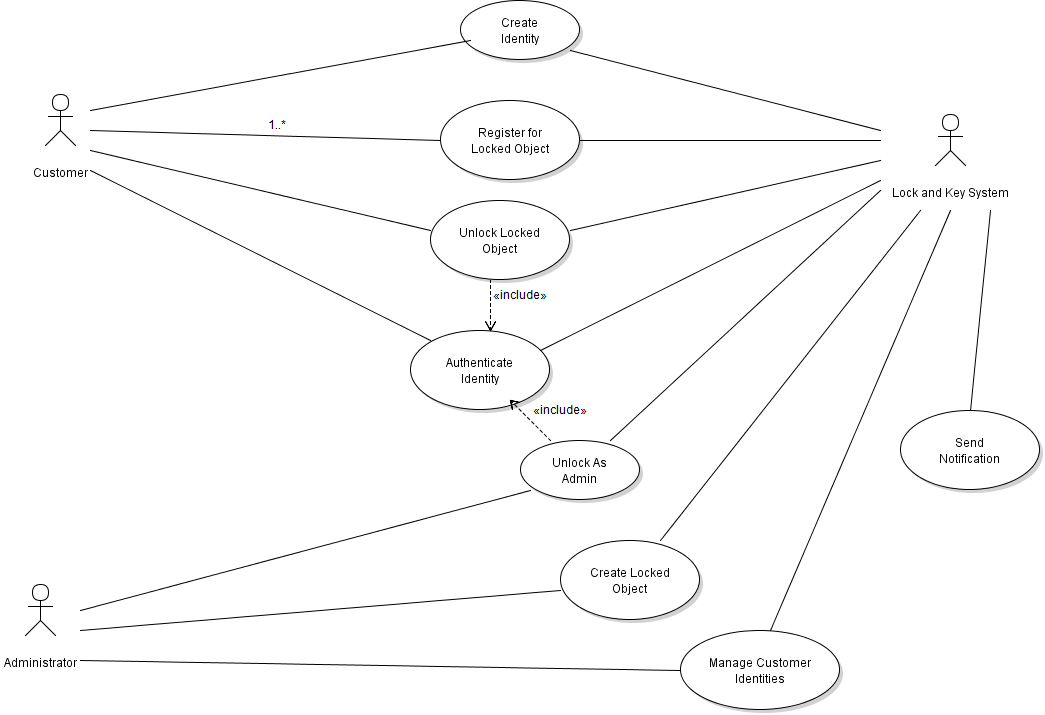
\includegraphics[width=\textwidth]{UML/lock_and_key}
	\caption{Use case diagram}
	\label{fig:use_case}
\end{figure}

\end{appendices}

\pagebreak

\printbibliography

\end{document}
